% Options for packages loaded elsewhere
\PassOptionsToPackage{unicode}{hyperref}
\PassOptionsToPackage{hyphens}{url}
%
\documentclass[
  man,floatsintext]{apa6}
\usepackage{amsmath,amssymb}
\usepackage{iftex}
\ifPDFTeX
  \usepackage[T1]{fontenc}
  \usepackage[utf8]{inputenc}
  \usepackage{textcomp} % provide euro and other symbols
\else % if luatex or xetex
  \usepackage{unicode-math} % this also loads fontspec
  \defaultfontfeatures{Scale=MatchLowercase}
  \defaultfontfeatures[\rmfamily]{Ligatures=TeX,Scale=1}
\fi
\usepackage{lmodern}
\ifPDFTeX\else
  % xetex/luatex font selection
\fi
% Use upquote if available, for straight quotes in verbatim environments
\IfFileExists{upquote.sty}{\usepackage{upquote}}{}
\IfFileExists{microtype.sty}{% use microtype if available
  \usepackage[]{microtype}
  \UseMicrotypeSet[protrusion]{basicmath} % disable protrusion for tt fonts
}{}
\makeatletter
\@ifundefined{KOMAClassName}{% if non-KOMA class
  \IfFileExists{parskip.sty}{%
    \usepackage{parskip}
  }{% else
    \setlength{\parindent}{0pt}
    \setlength{\parskip}{6pt plus 2pt minus 1pt}}
}{% if KOMA class
  \KOMAoptions{parskip=half}}
\makeatother
\usepackage{xcolor}
\usepackage{graphicx}
\makeatletter
\def\maxwidth{\ifdim\Gin@nat@width>\linewidth\linewidth\else\Gin@nat@width\fi}
\def\maxheight{\ifdim\Gin@nat@height>\textheight\textheight\else\Gin@nat@height\fi}
\makeatother
% Scale images if necessary, so that they will not overflow the page
% margins by default, and it is still possible to overwrite the defaults
% using explicit options in \includegraphics[width, height, ...]{}
\setkeys{Gin}{width=\maxwidth,height=\maxheight,keepaspectratio}
% Set default figure placement to htbp
\makeatletter
\def\fps@figure{htbp}
\makeatother
\setlength{\emergencystretch}{3em} % prevent overfull lines
\providecommand{\tightlist}{%
  \setlength{\itemsep}{0pt}\setlength{\parskip}{0pt}}
\setcounter{secnumdepth}{-\maxdimen} % remove section numbering
% Make \paragraph and \subparagraph free-standing
\makeatletter
\ifx\paragraph\undefined\else
  \let\oldparagraph\paragraph
  \renewcommand{\paragraph}{
    \@ifstar
      \xxxParagraphStar
      \xxxParagraphNoStar
  }
  \newcommand{\xxxParagraphStar}[1]{\oldparagraph*{#1}\mbox{}}
  \newcommand{\xxxParagraphNoStar}[1]{\oldparagraph{#1}\mbox{}}
\fi
\ifx\subparagraph\undefined\else
  \let\oldsubparagraph\subparagraph
  \renewcommand{\subparagraph}{
    \@ifstar
      \xxxSubParagraphStar
      \xxxSubParagraphNoStar
  }
  \newcommand{\xxxSubParagraphStar}[1]{\oldsubparagraph*{#1}\mbox{}}
  \newcommand{\xxxSubParagraphNoStar}[1]{\oldsubparagraph{#1}\mbox{}}
\fi
\makeatother
% definitions for citeproc citations
\NewDocumentCommand\citeproctext{}{}
\NewDocumentCommand\citeproc{mm}{%
  \begingroup\def\citeproctext{#2}\cite{#1}\endgroup}
\makeatletter
 % allow citations to break across lines
 \let\@cite@ofmt\@firstofone
 % avoid brackets around text for \cite:
 \def\@biblabel#1{}
 \def\@cite#1#2{{#1\if@tempswa , #2\fi}}
\makeatother
\newlength{\cslhangindent}
\setlength{\cslhangindent}{1.5em}
\newlength{\csllabelwidth}
\setlength{\csllabelwidth}{3em}
\newenvironment{CSLReferences}[2] % #1 hanging-indent, #2 entry-spacing
 {\begin{list}{}{%
  \setlength{\itemindent}{0pt}
  \setlength{\leftmargin}{0pt}
  \setlength{\parsep}{0pt}
  % turn on hanging indent if param 1 is 1
  \ifodd #1
   \setlength{\leftmargin}{\cslhangindent}
   \setlength{\itemindent}{-1\cslhangindent}
  \fi
  % set entry spacing
  \setlength{\itemsep}{#2\baselineskip}}}
 {\end{list}}
\usepackage{calc}
\newcommand{\CSLBlock}[1]{\hfill\break\parbox[t]{\linewidth}{\strut\ignorespaces#1\strut}}
\newcommand{\CSLLeftMargin}[1]{\parbox[t]{\csllabelwidth}{\strut#1\strut}}
\newcommand{\CSLRightInline}[1]{\parbox[t]{\linewidth - \csllabelwidth}{\strut#1\strut}}
\newcommand{\CSLIndent}[1]{\hspace{\cslhangindent}#1}
\ifLuaTeX
\usepackage[bidi=basic]{babel}
\else
\usepackage[bidi=default]{babel}
\fi
\babelprovide[main,import]{english}
% get rid of language-specific shorthands (see #6817):
\let\LanguageShortHands\languageshorthands
\def\languageshorthands#1{}
% Manuscript styling
\usepackage{upgreek}
\captionsetup{font=singlespacing,justification=justified}

% Table formatting
\usepackage{longtable}
\usepackage{lscape}
% \usepackage[counterclockwise]{rotating}   % Landscape page setup for large tables
\usepackage{multirow}		% Table styling
\usepackage{tabularx}		% Control Column width
\usepackage[flushleft]{threeparttable}	% Allows for three part tables with a specified notes section
\usepackage{threeparttablex}            % Lets threeparttable work with longtable

% Create new environments so endfloat can handle them
% \newenvironment{ltable}
%   {\begin{landscape}\centering\begin{threeparttable}}
%   {\end{threeparttable}\end{landscape}}
\newenvironment{lltable}{\begin{landscape}\centering\begin{ThreePartTable}}{\end{ThreePartTable}\end{landscape}}

% Enables adjusting longtable caption width to table width
% Solution found at http://golatex.de/longtable-mit-caption-so-breit-wie-die-tabelle-t15767.html
\makeatletter
\newcommand\LastLTentrywidth{1em}
\newlength\longtablewidth
\setlength{\longtablewidth}{1in}
\newcommand{\getlongtablewidth}{\begingroup \ifcsname LT@\roman{LT@tables}\endcsname \global\longtablewidth=0pt \renewcommand{\LT@entry}[2]{\global\advance\longtablewidth by ##2\relax\gdef\LastLTentrywidth{##2}}\@nameuse{LT@\roman{LT@tables}} \fi \endgroup}

% \setlength{\parindent}{0.5in}
% \setlength{\parskip}{0pt plus 0pt minus 0pt}

% Overwrite redefinition of paragraph and subparagraph by the default LaTeX template
% See https://github.com/crsh/papaja/issues/292
\makeatletter
\renewcommand{\paragraph}{\@startsection{paragraph}{4}{\parindent}%
  {0\baselineskip \@plus 0.2ex \@minus 0.2ex}%
  {-1em}%
  {\normalfont\normalsize\bfseries\itshape\typesectitle}}

\renewcommand{\subparagraph}[1]{\@startsection{subparagraph}{5}{1em}%
  {0\baselineskip \@plus 0.2ex \@minus 0.2ex}%
  {-\z@\relax}%
  {\normalfont\normalsize\itshape\hspace{\parindent}{#1}\textit{\addperi}}{\relax}}
\makeatother

\makeatletter
\usepackage{etoolbox}
\patchcmd{\maketitle}
  {\section{\normalfont\normalsize\abstractname}}
  {\section*{\normalfont\normalsize\abstractname}}
  {}{\typeout{Failed to patch abstract.}}
\patchcmd{\maketitle}
  {\section{\protect\normalfont{\@title}}}
  {\section*{\protect\normalfont{\@title}}}
  {}{\typeout{Failed to patch title.}}
\makeatother

\usepackage{xpatch}
\makeatletter
\xapptocmd\appendix
  {\xapptocmd\section
    {\addcontentsline{toc}{section}{\appendixname\ifoneappendix\else~\theappendix\fi: #1}}
    {}{\InnerPatchFailed}%
  }
{}{\PatchFailed}
\makeatother
\keywords{fairtheory, meta theory, theory formation, cumulative science, formal models\newline\indent Word count: 8688}
\usepackage{lineno}

\linenumbers
\usepackage{csquotes}
\ifLuaTeX
  \usepackage{selnolig}  % disable illegal ligatures
\fi
\usepackage{bookmark}
\IfFileExists{xurl.sty}{\usepackage{xurl}}{} % add URL line breaks if available
\urlstyle{same}
\hypersetup{
  pdftitle={FAIR theory: Applying Open Science Principles to the Construction and Iterative Improvement of Scientific Theories},
  pdfauthor={Caspar J. Van Lissa1, Aaron Peikert2,3, Andreas M. Brandmaier2,3,4, Felix D. Schönbrodt5, \& Noah N.N. van Dongen6},
  pdflang={en-EN},
  pdfkeywords={fairtheory, meta theory, theory formation, cumulative science, formal models},
  hidelinks,
  pdfcreator={LaTeX via pandoc}}

\title{FAIR theory: Applying Open Science Principles to the Construction and Iterative Improvement of Scientific Theories}
\author{Caspar J. Van Lissa\textsuperscript{1}, Aaron Peikert\textsuperscript{2,3}, Andreas M. Brandmaier\textsuperscript{2,3,4}, Felix D. Schönbrodt\textsuperscript{5}, \& Noah N.N. van Dongen\textsuperscript{6}}
\date{}


\shorttitle{FAIR THEORY}

\authornote{

This is a preprint paper, generated from Git Commit \# c910eaa6.

The authors made the following contributions. Caspar J. Van Lissa: Conceptualization, Formal Analysis, Funding acquisition, Methodology, Project administration, Software, Supervision, Writing -- original draft, Writing -- review \& editing; Aaron Peikert: Formal Analysis, Writing -- original draft, Writing -- review \& editing; Andreas M. Brandmaier: Formal Analysis, Writing -- original draft, Writing -- review \& editing; Felix D. Schönbrodt: Conceptualization, Writing -- review \& editing; Noah N.N. van Dongen: Writing -- review \& editing.

Correspondence concerning this article should be addressed to Caspar J. Van Lissa, Professor Cobbenhagenlaan 125, 5037 DB Tilburg, The Netherlands. E-mail: \href{mailto:c.j.vanlissa@tilburguniversity.edu}{\nolinkurl{c.j.vanlissa@tilburguniversity.edu}}

}

\affiliation{\vspace{0.5cm}\textsuperscript{1} Tilburg University, dept. Methodology \& Statistics\\\textsuperscript{2} Center for Lifespan Psychology, Max Planck Institute for Human Development, Berlin, Germany\\\textsuperscript{3} Max Planck UCL Centre for Computational Psychiatry and Ageing Research, Berlin, Germany\\\textsuperscript{4} Department of Psychology, MSB Medical School Berlin, Berlin, Germany\\\textsuperscript{5} Ludwig-Maximilians-Universität München, Germany\\\textsuperscript{6} University of Amsterdam, the Netherlands}

\abstract{%
Test test.
}



\begin{document}
\maketitle

The FAIR Guiding Principles (hereafter: FAIR principles) were established to improve the reusability of research data by making them more findable, accessible, interoperable and reusable {[}REF{]} for both humans and computers.
Since their inception in 2014, scholars have demonstrated their relevance for making other information artefacts more open, such as research software (Lamprecht et al., 2019) and computational workflows (S. R. Wilkinson et al., 2024).
This paper argues that the FAIR principles can advance effective and transparent scholarly communication about theory.
To this end, we introduce ``FAIR theory'':
a digital instantiation of a scientific theory, published as a self-contained and citable information artifact distinct from the scientific paper,
compliant with the FAIR principles.
FAIR theory has the potential to improve the efficiency of scholarly communication and
accelerate cumulative knowledge acquisition.

\subsection{The Need for FAIR theory}\label{the-need-for-fair-theory}

The so-called ``replication crisis'' has prompted extensive reforms in social science (Lavelle, 2021; Scheel, 2022).
Concern that undisclosed flexibility in analyses was a major factor for the abundance of non-replicable findings led to widespread adoption of open science practices like preregistration and replication (Nosek et al., 2015).
These various practices ensure transparent and repeated testing of hypotheses.
However, recent reviews show that most preregistered hypothesis tests are not supported by empirical evidence (Scheel, Schijen, \& Lakens, 2021).
Thus, increased rigor in testing has revealed that the root cause of the replication crisis is more fundamental:
Psychological theories rarely provide hypotheses that are corroborated by evidence.
Furthermore, theories are often so vague that they can accommodate mutually inconsistent findings,
as the theory's central claims evade falsification.

Scholars have been raising concerns about the state of theory in social science for nearly 50 years (Paul E. Meehl, 1978; Robinaugh, Haslbeck, Ryan, Fried, \& Waldorp, 2021).
One main concern is that social scientific theories lack precision, or \emph{formalization} (Szollosi \& Donkin, 2021).
When theories do not make precise predictions,
they are hard to falsify and difficult to understand on their own,
without either substantial interpretation or additional background knowledge.
A second concern is the lack of transparent and participative scholarly communication about psychological theory, which limits its progression and development.

Given these concerns, it is an imbalance that scientific reform initiated by the open science movement has focused primarily on improving deductive methods.
The equally critical inductive processes of theory construction and theory improvement have been largely overlooked\footnote{We use induction to describe inferences from specific observations to general theories; others have coined \emph{abduction} to describe ``inference to the best explanation'' {[}REF Peirce{]}. However, Peirce also acknowledged that abduction ``is not essentially different from induction'' (p.4481). Defining what makes a theory ``best'' requires making auxiliary assumptions. For present purposes, induction and abduction are interchangeable terms.}.
The present paper restores balance by applying, for the first time,
open science principles to psychological theory.
We apply the FAIR principles to scientific theories,
introducing the concept of \emph{FAIR theory} to
facilitate transparent scholarly communication and accelerate cumulative knowledge acquisition.

\subsection{Theory and Scientific Progress}\label{theory-and-scientific-progress}

According to the \emph{empirical cycle} (de Groot, 1961),
a meta-theoretical model of cumulative knowledge acquisition,
research ideally follows a cyclical process with two phases (Figure \ref{fig:figec}).
In the deductive phase, hypotheses derived from theory are tested on data. In the inductive phase, patterns observed in data are generalized to theoretical principles.
In this model, theories are the vehicle of scientists' understanding of phenomena.
Ideally, they are iteratively updated based on deductive testing and inductive theory construction.

\begin{figure}
\centering
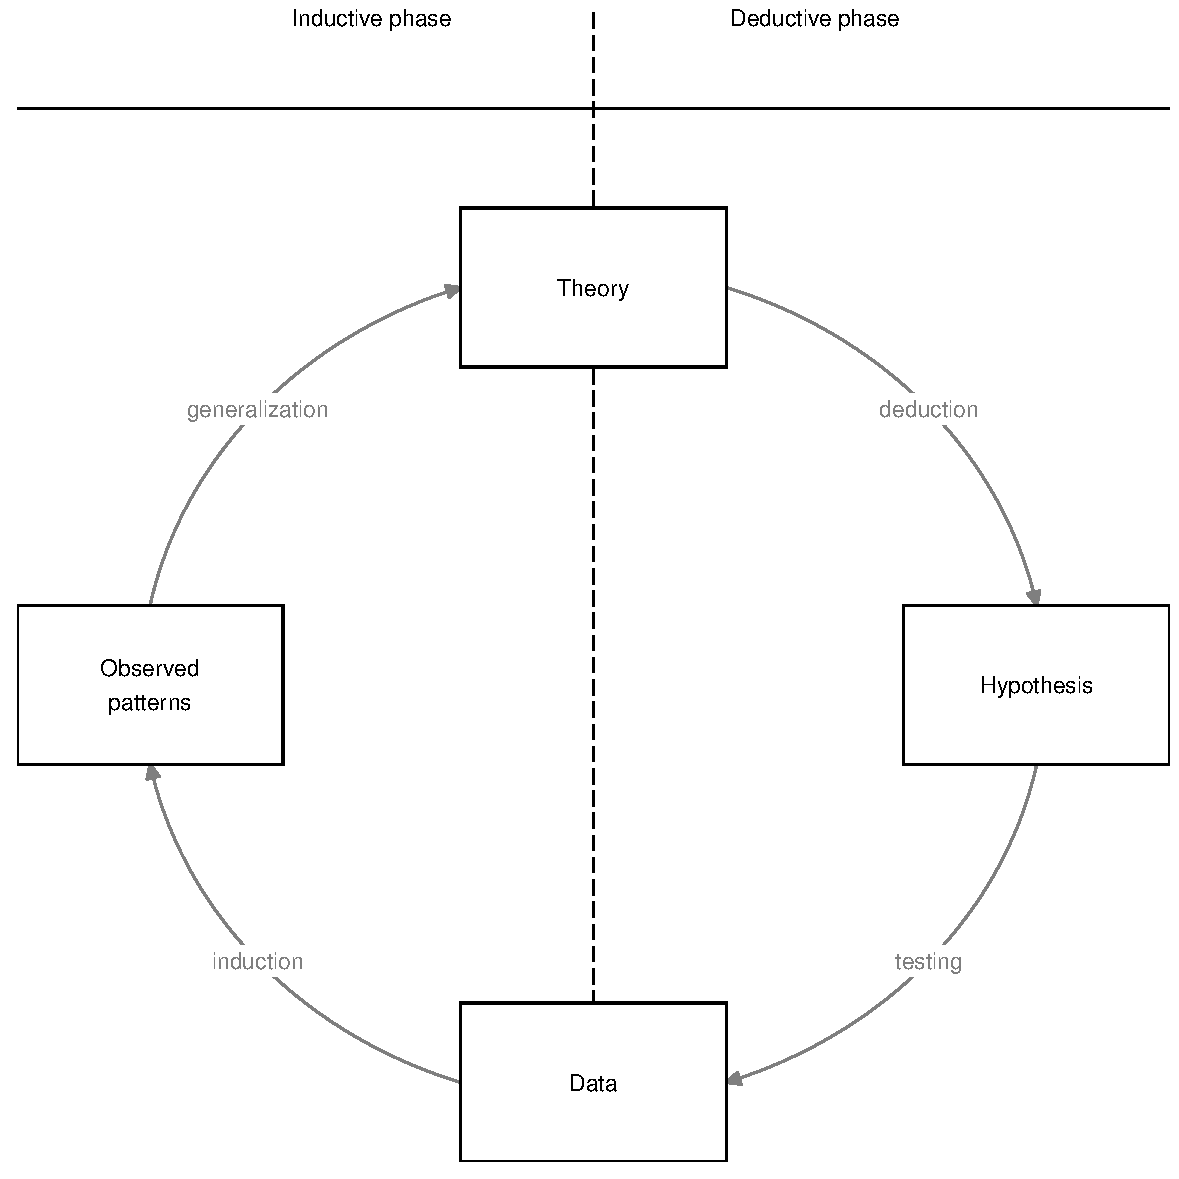
\includegraphics{empirical_cycle.pdf}
\caption{\label{fig:figec}A take on the empirical cycle by De Groot}
\end{figure}

In a progressive research program (Lakatos, 1971),
this cycle is regularly completed to iteratively advance our understanding of the studied phenomena
.
There are, however, indications that contemporary psychology falls short of this ideal.
Firstly, because hypothesis-testing research is over-represented in the literature:
According to Kühberger, Fritz, and Scherndl (2014), 89.6\% of papers published in psychology report confirmatory hypothesis tests.
In addition, the link between theory and hypothesis is often tenuous or absent (Oberauer \& Lewandowsky, 2019; Scheel, Tiokhin, Isager, \& Lakens, 2021).
Only 15\% of deductive studies referenced any theory, and theory was often not cited in relation to the hypothesis (McPhetres et al., 2021).
The remaining 85\% of deductive studies lacked an explicit connection between theory and hypothesis.
In the best case, such ungrounded hypotheses are rooted in researchers' implicit theories, in which case it is particularly important to make these explicit Norouzi, Kleinberg, Vermunt, \& Van Lissa (2024).
Or, perhaps the hypotheses are not of substantive interest, such as null hypotheses that exist purely for the purpose of being rejected (Van Lissa et al., 2020), and researchers are simply testing them as part of a cultural ritual (Gigerenzer, Krauss, \& Vitouch, 2004).
Testing ad-hoc hypotheses not grounded in theory does not advance our principled understanding of psychological phenomena.
Put differently: collecting significance statements about ad-hoc hypotheses is much like trying to write novels by collecting sentences from randomly generated letter strings (van Rooij \& Baggio, 2021).

Theory thus has an uncomfortable and paradoxical role in contemporary psychology:
The majority of papers ostensibly test hypotheses,
but these are rarely connected, let alone derived, from theory,
and test results do not routinely reference back to theories, contributing to their improvement or rejection.
The paradoxical role of theory in psychology is perhaps best described by Meehl's observation that theories in psychology ``lack the cumulative character of scientific knowledge. They tend neither to be refuted nor corroborated, but instead merely fade away as people lose interest'' (Paul E. Meehl, 1978).

\subsection{Making Theory FAIR}\label{making-theory-fair}

The present paper addresses the lack of open science methods for theory development and suggests an improvement of the state of affairs by applying the FAIR principles to scientific theories.
Merely publishing theory in a research article does not make it open;
to be open, theory should adhere to established open science standards.
We apply the FAIR principles to digital representations of theory,
introducing a FAIR metadata format to make theories \emph{Findable} via a DOI,
\emph{Accessible} in a machine- and human-readable filetype,
\emph{Interoperable} within the data analysis environment,
and \emph{Reusable} in the practical and legal sense, so that they may be improved over time -- at best, in a participative process.
Digital representations of theory intentionally is a broad term, particularly including textual representations of a given theory, as well as formal representations, such as mathematical notation, algorithmic pseudo code, or a set of logical clauses.
Following the original proposal of Lamprecht and colleagues,
we adapt the FAIR principles for theory, see Table \ref{tab:tabfair}.
We reflect on the necessary changes (which are minor),
as well as on the current state and future of FAIR theory in the social sciences.
The resulting principles provide guidance for instantiating theory as a FAIR information artifact,
and we provide worked examples to encourage their adoption.

\begin{lltable}

\begin{longtable}{m{.1\linewidth}m{.35\linewidth}m{.35\linewidth}m{.15\linewidth}m{.1\linewidth}m{.35\linewidth}m{.35\linewidth}m{.15\linewidth}m{.1\linewidth}m{.35\linewidth}m{.35\linewidth}m{.15\linewidth}m{.1\linewidth}m{.35\linewidth}m{.35\linewidth}m{.15\linewidth}}\noalign{\getlongtablewidth\global\LTcapwidth=\longtablewidth}
\caption{\label{tab:tabfair}}\\
\toprule
Criterion & \multicolumn{1}{c}{Original} & \multicolumn{1}{c}{Theory} & \multicolumn{1}{c}{Action}\\
\midrule
\endfirsthead
\caption*{\normalfont{Table \ref{tab:tabfair} continued}}\\
\toprule
Criterion & \multicolumn{1}{c}{Original} & \multicolumn{1}{c}{Theory} & \multicolumn{1}{c}{Action}\\
\midrule
\endhead
F1 & (Meta)data are assigned a globally unique and persistent identifier & Theory (meta)data has a global, unique and persistent identifier & Rephrased\\
F2 & Data are described with rich metadata & Theory is described with rich metadata & Rephrased\\
F3 & Metadata clearly and explicitly include the identifier of the data it describes & Metadata clearly and explicitly include identifiers for all the versions of the theory it describes & Rephrased and extended\\
F4 & (Meta)data are registered or indexed in a searchable resource & Theory and its associated metadata are included in a searchable repository & Rephrased, needs work\\
A1 & (Meta)data are retrievable by their identifier using a standardized communications protocol & Theory and its associated metadata are accessible by their identifier using a standardized communications protocol & Rephrased\\
A1.1 & The protocol is open, free, and universally implementable & The protocol is open, free, and universally implementable & Remain the same\\
A1.2 & The protocol allows for an authentication and authorization procedure, where necessary & The protocol allows for an authentication and authorization procedure, where necessary & Remain the same, but less relevant\\
A2 & Metadata are accessible, even when the data are no longer available & Theory metadata are accessible, even when the theory is no longer available & Rephrased, but less relevant\\
I1 & (Meta)data use a formal, accessible, shared, and broadly applicable language for knowledge representation & Theory and its associated metadata use a formal, accessible, shared and broadly applicable language to facilitate machine readability and reuse & Rephrased and extended\\
I2 & (Meta)data use vocabularies that follow FAIR principles & (Meta)data use vocabularies that follow FAIR principles & Rephrased\\
I2S.1 & - &  & \\
I2S.2 & - &  & \\
I3 & (Meta)data include qualified references to other (meta)data & (Meta)data includes qualified references to other (meta)data, including previous versions of the theory & Extended\\
I4S & - &  & \\
R1 & (Meta)data are richly described with a plurality of accurate and relevant attributes & Theory and its associated metadata are richly described with a plurality of accurate and relevant attributes & Rephrased\\
R1.1 & (Meta)data are released with a clear and accessible data usage license & Theory (meta)data are released with a clear and accessible license & Rephrased\\
R1.2 & (Meta)data are associated with detailed provenance & Theory (meta)data are associated with detailed provenance & Rephrased\\
R1.3 & (Meta)data meet domain-relevant community standards & Theory (meta)data and documentation meet domain-relevant community standards & Rephrased\\
\bottomrule
\end{longtable}

\end{lltable}

\subsection{What is Theory?}\label{what-is-theory}

Definitions of theory abound and are the subject of extensive scholarly debate.
Given that a pluriformity of definitions are consistent with FAIR theory principles,
our paper is not aligned with one particular definition.
Perspectives on scientific theory have been categorized as syntactic, semantic, and pragmatic (Winther, 2021)
The syntactic view describes theories as ``sets of sentences in a given logical domain language'' (Winther, 2021, ch.~2),
acknowledging that each domain (a scientific field, such as psychology or physics) has its own theoretical vocabulary.
We recognize the syntactic view in Meehl's hierarchy of ever-more specific ``statements'' a theory might contain (1990):
statements about the types of entities postulated (i.e., ontology),
statements about causal connections between those entities,
statements about the functional form of those connections,
and statements about their specific numerical values Guest (2024).

The semantic view challenges the necessity of distinct domain languages for different scientific fields, and instead advocates for formalizing theories using mathematics.
It shifts the focus from theories as collections of sentences to mathematical models.
The term ``model'' is not uniquely defined within the literature;
it has been described as a ``specific instantiation of theory narrower in scope and often more concrete, commonly applied to a particular aspect of a given theory'' {[}REF Fried{]}.
This implies that theories and models are not fundamentally distinct, but rather, that for each model, there is a more general theory that subsumes it (one person's model is another person's theory).
-

The pragmatic view holds that there might not be one structure or definition of scientific theories, but instead, definitions differ across scientific domains.
It also argues that nonformal aspects (e.g.~commonly used analogies) and practices (e.g.~experimental designs) can be an important part of scientific theories.

Since the primary purpose of FAIR theories is to advance scholarly communication about theories,
the method is not contained to any one particular definition.
It is best left to the scholarly community to decide which parts of theory, models, or other aspects should be represented as FAIR theory.
As the practice of FAIRification becomes more embedded,
we expect that it will become increasingly clear what kind and form of information is useful.
As a particular FAIR theory evolves, the nature of the information tracked will likely change.
For example, following Meehl, we could envision a theory that starts out specifying how specific constructs are causally connected.
From this theory, more precise \emph{statistical/mathematical models} could be derived by the theory's suggestions for functional form (e.g., linear effects) and error families (e.g., normal distributions).
This statistical model makes just enough assumptions to allow the estimation of the remaining unknown parameters (e.g., regression slopes) from data.
Then, an even more specific \emph{generative/computational model} could be added, which is completely parameterized (i.e., specific values of regression slopes are also assumed) such that an interpreter (e.g., the R programming language) can use the model to generate new data.
Also, aspects of scientific practice might be added over time, such as commonly used experimental designs (e.g.~longitudinal designs observing change over time), measurement tools (e.g.~different questionnaires used to assess the same construct), or study subjects (e.g.~specific strains of rats).

As an applied example, consider a comprehensive theory of disease spread and pandemics which covers various psychological factors such as adherence to pandemic mitigation methods (e.g., ), pandemic-related social disruption (e.g., panic buying), or pandemic-related distress and related problems (e.g., anxiety) (Taylor, 2022).
The theory may encompass a particular transmission \emph{model} for disease spread including precise parameters for the process of infection (e.g., social distance, average duration of encounters, ventilation) and incubation times.

\subsubsection{The Role of Theory Formalization}\label{the-role-of-theory-formalization}

Concerns about the state of theory in the psychological literature revolve around two issues: theory formalization and theory (re-)use.
Greater formalization increases theories' \emph{empirical content} {[}REF{]} because it expresses ideas as precise statements, clearly demarcating what should (not) be observed.
For example, Baddeley's verbal description of the phonological loop in his theory of working memory allows for at least 144 different implementations depending on the specification of the decay rate, recall success, or rehearsal sequence (Lewandowsky \& Farrell, 2010).
Without committing to specific implementations a-priori,
the theory becomes hard to test.
Committing to specific implementations of the different components, their causal connections, and the functional forms of these relationships makes the theory more precise.
More precise theories are easier to falsify,
which necessitates specific revisions and advances our principled understanding of the phenomena they describe.

Although we are in favor of the advancement towards formal theories,
this might not always be desirable or feasible.
Fortunately, formalization is not required to make theories FAIR.
To some extent, FAIRness and formalization are orthogonal.
FAIR theory imposes no restrictions on the manner in which theories are derived and implemented;
rather, it increases the fidelity and ease with which they are communicated.
The FAIR principles pertain to theories' documentation, archival, and sharing in digital environments, with the aim of enhancing their reusability and extensibility.
For example, a collection of verbal propositions derived through qualitative research could be represented as a FAIR theory.
Conversely, a formal theory is not FAIR if it is represented as a bitmap image in a journal article without any key words to identify it as a theory paper to search engines.
FAIR theory is thus consistent with, but does not require, formalization (also see \emph{Accessibility}).

\subsubsection{Modular Publishing}\label{modular-publishing}

We propose FAIR theory as an instantiation of modular publishing (\textbf{kirczModularityNextForm1998?}).
At present, the primary unit of social scientific communication is the academic paper.
A paper may depend on multiple resources - materials, data, code, and theory - but these are often merely described in the text.
Modular publishing is the practice of making each of these resources available as independent citable \emph{information artifacts} in their own right,
with adequate metadata that is indexed in standardized repositories (\textbf{vandesompelRethinkingScholarlyCommunication2004?}).
Data sharing is a good example of a modular publishing practice that is widely adopted and increasingly required by funding agencies, journals, and universities.
Scholars can archive information artifacts in repositories like \href{https://zenodo.org/}{Zenodo},
which was developed by \href{https://home.cern/}{CERN} under the European Union's \href{https://www.openaire.eu/}{OpenAIRE} program.
To maintain a persistent record of scholarly communication,
Zenodo mints DOIs for information artifacts - as does, for example, the \href{https://www.crossref.org/}{Crossref} association,
which is used by many academic publishers.
Finally, the \href{}{DataCite Metadata Schema} offers a standard way to document the nature of relationships between information artifacts.
For example, a dataset collected for a specific paper would be archived in Zenodo with the metadata property \texttt{resourceType:\ dataset},
and cross-reference the published paper with \texttt{relationType:\ IsSupplementTo}.
Similarly, FAIR theories can be connected to a specific paper which might serve as the theory's documentation and canonical reference.

\subsubsection{Version Control}\label{version-control}

We can take inspiration from the field of computer science for well-established processes for iteratively improving information artifacts.
Version control systems, like Git, have long been used to iteratively improve computer code, while managing parallel contributions and allowing for diverging development.
Git tracks line-by-line changes to text-based files,
and maintains a complete history of those changes.
It has long been argued that Git is particularly well-suited to academic work (Ram, 2013).
Git can be used, for example, to facilitate reproducible research, manage distributed collaboration, and improve preregistration (Peikert, Van Lissa, \& Brandmaier, 2021; Van Lissa et al., 2021).
The present paper considers the advantages of Git for FAIR theory.
Git enables explicitly comparing versions of a file (or: theory),
incorporating changes by different authors,
and branching off into different directions (e.g., competing hypotheses) while retaining an explicit link to the common ancestor.
This makes it possible for meta-scientists to study the provenance of a theory and determine how well different versions of a theory explain empirical evidence (Van Lissa, 2023).

\subsubsection{Semantic Versioning}\label{semantic-versioning}

Aside from technical solutions, version control is a social process as well.
On the one hand, regular updates can improve theories - but on the other hand, it risks breaking compatibility between theories and hypotheses derived from them, or compatibility between one theory and others that depend upon it.
For example, if we construct a theory to explain a specific phenomenon, and we cross-reference an existing theory comprising an ontology for our field - that dependency is broken if the ontology is later updated and our phenomenon of interest is removed.
In computer science, these challenges are navigated by assigning version numbers.
Specifically, \emph{semantic versioning} comprises a simple set of rules for assigning version numbers to information artifacts.
Whereas version control tracks changes,
semantic versioning communicates what those changes mean to users of the theory.
We propose the following adaptation of semantic versioning for theories:

\begin{verbatim}
Given a version number MAJOR.MINOR.PATCH, increment the:

MAJOR version when you make backwards incompatible changes, i.e., the theory now contains empirical statements that are at odds with a previous version
MINOR version when you expand the set of empirical statements in a backward compatible manner (i.e., the previous version is subsumed within the new version)
PATCH version when you make backward compatible bug fixes,
cosmetic changes, fix spelling errors, or add clarifications
\end{verbatim}

Semantic versioning guides the social process of theory development, communicating how much a theory is changing over tiem.

\section{The FAIR Principles}\label{the-fair-principles}

\subsection{Findability}\label{findability}

Making theories Findable would allow researchers to easily identify relevant theories to inform their hypotheses,
grounding their work in established theoretical foundations.
It further increases the impact and reuse potential of theories across disciplines,
either through direct application (where one discipline stumbles upon a problem that is already well-understood in another discipline),
or through analogical modeling.
In analog modeling, the structure of a theory from one discipline is applied to a phenomenon in another field.
For example, predator-prey models have inspired theories of XXX, and the Eysenck model of atomic magnetism has inspired a network theory of depression.
Findability also enables meta-research on theories,
in the same way libraries and search engines have enabled scholars to study the literature via systematic reviews.
In a similar way, it would become much easier to explicitly compare different theories of a specific phenomenon,
or to study structural properties of theories.

The four Findability criteria are applicable to theory with only minor adjustments, see Table \ref{tab:tabfair}.
First, this requires assigning a globally unique and persistent identifier, or DOI, to each theory (F1).
Of the many services that provide DOIs for scientific information artefacts,
Zenodo and the Open Science Framework are commonly used in psychology.
Second, Findable theory is described with rich metadata (F2).
This includes citation metadata (e.g., referencing a scientific paper that documents the theory, or a psychometric paper that operationalizes specific constructs).
It might further include domain-specific metadata, such as a reference to a taxonomy of psychological constructs (Bosco, Uggerslev, \& Steel, 2017),
ontology (Guyon, Kop, Juhel, \& Falissard, 2018),
or catalog of psychological phenomena {[}REF Noah Denny{]}.
Metadata should also include identifiers for all the versions of the theory it describes (F3);
Zenodo handles this by default by providing an overarching DOI for an information artifact which subsumes the DOIs of that artifact's versions.

Finally, metadata should be registered or indexed in a searchable registry (F4).
Zenodo and GitHub are both searchable.
Standardized metadata further enhance Findability in these repositories.
The DataCite Metadata Schema provides a controlled vocabulary for research output, and the \texttt{resource\_type:\ model} matches the description of FAIR theory (\textbf{datacitemetadataworkinggroupDataCiteMetadataSchema2024?}).
Furthermore, a standard keyword can be used; we suggest using the keyword \texttt{"fairtheory"} for all resources that constitute or reference a FAIR theory.

Findability is substantially amplified if intended users of a resource know where to search for it.
This is a known problem in relation to research data and software (\textbf{katzSpecialIssueSoftware2024?}).
Regrettably, most academic search engines are designed to index traditional print publications, not other information artifacts.
Since the status quo is to publish theories in papers,
the FAIR requirements are met if scholars continue to do so,
and additionally publish theories as separate information artifacts.
The \texttt{"fairtheory"} keyword can also be used to signal the presence of theory within a paper.
In the longer term, it may not be necessary to write a paper for each theory.
If Zenodo becomes more recognized as centralized repository for information artifacts, researchers may begin to search there more regularly.
Conversely, as organizations begin to recognize the value in tracking academic output other than papers, repositories may begin to index information artifacts stored in Zenodo.

There have been notable efforts to improve theories' findability through post-hoc curation.
For example, Gray and colleagues introduced a format for representing theories,
and post many examples on their website (Gray, 2017).
Similarly, Borsboom and colleagues seek to establish a database of psychological theories {[}REF BORSBOOM{]}.
Post-hoc curation is a notable effort but does not address the root cause of the lack of Findability, however.
Ideally, Findability would be addressed ante-hoc, through documentation with rich metadata and modular publishing.

\subsection{Accessibility}\label{accessibility}

Transparent scholarly communication about theory requires that theories are accessible to all researchers and other stakeholders.
If theories are accessible, researchers can reuse and refine them,
thus accelerating cumulative knowledge acquisition.
Making theories accessible also allows stakeholders (e.g., practitioners, policy makers, advocates) to inform themselves of the current scientific understanding of specific phenomena.
While isolated empirical findings can appear fragmented and contradictory (Dumas-Mallet, Smith, Boraud, \& Gonon, 2017),
theories offer a top-down, big picture representation of the phenomena studied in a field.
In other words, theories are an important instrument in science communication.

The Accessibility principles pertain to \emph{regulating} access, not only maximizing it.
They apply to theory with minor changes.
Firstly, theory and its associated metadata should be accessible by their identifier using a standardized communications protocol (A1).
This can be achieved, for example, by hosting theory in a version-controlled remote repository (such as git), and archiving that repository on Zenodo for long-term storage.
The resulting resource will then have an identifier (DOI) which allows the theory to be accessed using a standardized communications protocol (download via \texttt{https} or \texttt{git}).
Secondly (A2), theory metadata should be accessible, even when the theory is no longer available,
which is also achieved via long-term storage (e.g., on Zenodo).
Git remote repositories allow for access control,
and Zenodo allows for access control of individual files/resources.
In general, it makes sense to retain outdated theories, in order to be able to track the genesis of theories over time, yet, we require the availability of meta data as a minimum requirement.

At present, there are several impediments to theories' accessibility.
To the extent that theories are still contained within papers,
paywalls erected by commercial publishers constitute a barrier.
Open Access publishing thus increases the accessibility of all academic output, including theory.
A second impediment is more indirect:
While open access publishing increases practical access to theories,
accessibility also requires clear and explicit communication.
This property of good theories has been dubbed ``discursive survival {[}\ldots{]}, the ability to be understood'' (Guest, 2024).
At present, psychological theories are often ambiguous, rendering them difficult to understand (Frankenhuis et al., 2023).
It is important to acknowledge the \emph{indeterminacy of translation} (Quine, 1970):
which holds that every communicative utterance has multiple alternative translations, with no \emph{objective} means of choosing the correct one.
It follows that an idea cannot be formalized to the point that it becomes unambiguously interpretable.
This places a theoretical upper bound on theories' ability to be understood.

Successful communication requires shared background knowledge between sender and receiver (Vogt et al., 2024).
The Kuhnian notion of ``normal science'', conducted within the context of a shared paradigm, provides shared background knowledge to facilitate mutual understanding (Kuhn, 2009).
From a pragmatic perspective, these considerations indicate that,
when striving to make theory accessible,
it is important to be as explicit as possible (e.g., about assumptions and ontological definitions),
while acknowledging that accessibility exists on a spectrum,
and that it is impossible to eliminate all ambiguity.
Rather, it may benefit scientific discourse to anticipate misunderstanding,
and use it to drive further explication of theory.
In sum, efforts to communicate theory clearly, with as few dependencies on shared background knowledge as possible, including by formalization, explication of assumptions,
and cross-references to resources that provide relevant context (papers, ontologies, macro-theories, theories of measurement)
will advance its Accessibility.

A third impediment arises when theories have a ``dependency on the author'' (DOA).
DOA occurs when a theory cannot be understood by independent scholars,
thus requiring the original author for interpretation and clarification.
We have heard DOA referred to apocryphally as the ``ask Leon'' phenomenon,
as graduate students were supposedly told to ask Leon Festinger to explain to them how their misconstrual of cognitive dissonance theory had caused their experiments to yield null results.
DOA relates to the discourse on ``Great Man Theorizing'' (Guest, 2024) because it enables gatekeeping: an author could insist that work requires their involvement or denounce work conducted outside their purview as illegitimate,
which violates checks and balances of scientific research.
DOA also renders theories immune to refutation,
because the author can claim that the theory was misconstrued when confronted with falsifying evidence, thus making it a moving target (Szollosi \& Donkin, 2021).
The fact that DOA is inherently problematic is illustrated by cases where third parties identify logical inconsistencies within a theory (e.g., Kissner, 2008).
This demonstrates that original authors are not the ultimate authority on their theories.
DOA thus unduly impedes scientific progress, and authors should make good-faith efforts to make theories as accessible as possible in terms of both availability and interpretability.

\subsection{Interoperability}\label{interoperability}

Interoperability pertains to the property of information artefacts to ``integrate or work together {[}\ldots{]} with minimal effort'' (M. D. Wilkinson et al., 2016).
Firstly, theory and its associated metadata should use a formal, accessible, shared and broadly applicable language to facilitate (human- and) machine readability and reuse (I1).
The common practice of instantiating theory as lengthy prose or schematic drawing falls short of this ideal.
Instead, FAIR theory should, ad minimum,
be instantiated in a human- and machine-readable datatype,
as previously recommended (Van Lissa et al., 2021).
Depending on the level of formalization of the theory,
different formats may be appropriate,
such as verbal statements in plain text,
mathematical formulae,
and statements expressed in some formal language.
Examples of the latter include pseudo-code,
interpretable computer code,
and Gray's theory maps (Gray, 2017).
While a theory represented as a bitmap image is not very interoperable,
the same image represented in the DOT language (\textbf{DOTLanguage?}) for representing graphs does meet this ideal.

Secondly, theory (meta)data should use vocabularies that follow FAIR principles (I2).
Aside from the aforementioned Datacite metadata schema (\textbf{datacitemetadataworkinggroupDataCiteMetadataSchema2024?}),
in the context of theory, this highlights the importance of establishing standardized ontologies.
Thirdly, theory (meta)data should include qualified references to other (meta)data, including previous versions of the theory (I3).
The first part of this principle allows for nested theories;
for example, a theory that specifies causal relationships between constructs could refer back to an ontological theory from which those constructs are derived.
This can be achieved by cross-referencing the DOI of those nested theories ({``Contributing {Citations} and {References},''} n.d.).
The second part of this principle allows for tracing the provenance of a theory; keeping track of its prior versions and other theories that inspired it.
This is achieved by using Git for version control and Zenodo for archiving.
Git tracks the internal provenance of a theory repository; Zenodo is used to cross-reference external relationships (e.g., papers that influenced the theory, previous theories that inspired it, models based upon the theory).

Recent work points out that interoperability is not an all-or-nothing property.
The concept of X-interoperability was introduced to answer the question: \emph{interoperable for what?}
X-interoperability is defined as facilitating ``successful communication between machines and between humans and machines {[}, where{]} A and B are considered X-interoperable if a common operation X exists that can be applied to both'' (Vogt et al., 2024).
This revised definition makes it possible to outline a theory's affordances in terms of X-interoperability.
For example, a FAIR theory may be X-interoperable for deriving testable hypotheses,
or for the purpose of selecting relevant control variables,
or for the purpose of indicating the conditions necessary for observing a particular phenomenon.
If we consider Meehl's nine properties of strong theories (properties 3-8 are grouped because they all refer to functional form),
we see how each of these properties incurs certain affordances in terms of X-interoperability (Table \ref{tab:tabmeehl}).

\begin{table}[tbp]

\begin{center}
\begin{threeparttable}

\caption{\label{tab:tabmeehl}}

\begin{tabular}{ll}
\toprule
Property & \multicolumn{1}{c}{X-interoperability}\\
\midrule
1) Ontology & Variable selection\\
2) Causal connections & Model specification, covariate selection, causal inference\\
3-8) Functional Form & Deriving specific hypotheses\\
9) Numerical Value & Simulating data\\
\bottomrule
\end{tabular}

\end{threeparttable}
\end{center}

\end{table}

With regard to the state of interoperability in contemporary psychology,
Kurt Lewin's adage ``there's nothing as practical as a good theory'' (Lewin, 1943) implies that ought to be highly X-interoperable in psychological researchers' day-to-day work.
But, as we argued, this is not the case.
The examples of X-interoperability offered in Table \ref{tab:tabmeehl} illustrate that much can be gained by integrating theory directly into analysis workflows, and by making theory X-interoperable within software used for analysis.
For example, interoperable theory could be used
to select control variables for causal inference (Cinelli, Forney, \& Pearl, 2022),
or to preregister the inferential procedure that would lead to specific modifications of a theory after analyzing empirical data (Peikert et al., 2021),
or to derive machine-readable hypotheses (Lakens \& DeBruine, 2021) which could be automatically evaluated through integration testing (Van Lissa, 2023).
Furthermore, theories can be X-interoperable with each other to enable nesting, or using one theory to clarify elements of another theory.
For example, it should be possible to embed a theory about emotion regulation (e.g., Gross, 2015) within a theory of emotion regulation development (Morris, Silk, Steinberg, Myers, \& Robinson, 2007).

\subsection{Reusability}\label{reusability}

If we take cumulative knowledge acquisition to be a goal of scientific research, then Reusability is the ultimate purpose of making theory FAIR.
Applied to FAIR theory, reusability requires that theory and its associated metadata are richly described with a plurality of accurate and relevant attributes (R1) with a clear and accessible license for reuse (R1.1).
It should further have detailed provenance (R1.2),
which is achieved through version control with Git and archival on Zenodo.
Finally, the (meta)data which meets domain-relevant community standards (R1.3).
The Datacite metadata schema offers an initial template in this regard,
and this paper takes one step towards establishing more fine grained community standards for FAIR theory.

If we consider the current state of Reusability in psychological theory, there appears to be a norm \emph{against} theory reuse:
\emph{``{[}Theories are{]} like toothbrushes --- no self-respecting person wants to use anyone else's''} (Mischel, 2008).
As cumulative knowledge acquisition requires reusable theories that are continuously updated based on insights from new data, such a norm impedes scientific progress (de Groot, 1961).
In FAIR theory workshops, we similarly notice reluctance to reusing and adapting existing theories.
Students ask questions such as ``who owns theory'',
and ``who determines how a theory may be reused or changed''?
These questions imply a norm against modifying theory without consent from the author reminiscent of the aforementioned problem of dependency on the author.

Licensing theories for reuse unambiguously answers these questions.
With the caveat that legislation may vary across contexts and jurisdictions, the following should not be interpreted as legal advice.
In determining what license is appropriate for theory,
a key consideration is that copyright law protects authors' rights according to the \emph{idea-expression dichotomy} (Bently, Davis, \& Ginsburg, 2010).
It explicitly does not
\emph{``extend to any idea, procedure, process, system, method of operation, concept, principle, or discovery''}.
Copyright thus extends to creative works expressing a theory (e.g., writing, visual illustrations),
but not to the underlying theoretical idea.
It thus seems that theories expressed in prose or depicted visually - in other words, that fall short of the Accessibility criterion - are more likely to qualify for copyright protection than formal theories.
Another important consideration is that academic research is covered under ``fair use'' exemptions to copyright.
Given that copyright does not cover ideas in their purest form (like formal theories), and that academic use is likely exempted from its protection,
in many cases, it may be sensible to explicitly license theories in a way that encourages Reusability.
The CC0 (no rights reserved) license does this by explicitly waiving all rights and encouraging reuse.

Aside from legal conditions for reuse, there are also social considerations.
For example, while a CC0 license does not mandate attribution,
it is nonetheless essential that scholars comprehensively cite theory and related works to comply with established norms of attribution and comprehensive citation (Aalbersberg et al., 2018).
Another way to guide the social process of (diffuse) collaboration is to include a ``README'' file in the theory repository, which informs users about the ways in which they can reuse and contribute to a FAIR theory.
It is also possible to create or adopt a ``Code of Conduct'' which prescribes

\section{Making a Theory FAIR}\label{making-a-theory-fair}

Open science infrastructure is an area of active development, and as such,
the approach proposed here should not be considered definitive,
but rather, as one proposal for a FAIR-compliant implementation of theory.
The guiding principle of our implementation is to align and build upon existing successful open science infrastructures to the maximum possible extent.
At the time of writing (2024),
the value of using Git for version control of academic research is well-established,
and the integration of GitHub and Zenodo makes for a particularly user-friendly approach.
Zenodo and GitHub are also integrated with the Open Science Framework (OSF),
a popular platform in psychology.
Creating a front page on the OSF increases the visibility of a FAIR theory,
while the integration with Zenodo and GitHub removes the need for uploading and maintaining the same information on multiple platforms.
While we make use of specific open science infrastructures, it is important to stress that our workflow illustrates general principles which can also be implemented using other open science infrastructures.
The process described here can be largely automated in R using the \texttt{theorytools} package; see the package vignette on FAIR theory, \texttt{vignette("fairtheory",\ package\ =\ "theorytools")}.

\subsection{1. Implementing the Theory}\label{implementing-the-theory}

Given that we structured our argument around the importance of FAIR theory for cumulative knowledge production through scientific research around the \emph{empirical cycle},
we decided to use it as an example for this tutorial.
The resulting FAIR theory is available at \url{https://doi.org/10.5281/zenodo.14552329}.
The empirical cycle is described on page 28 of De Groot and Spiekerman (1969).
Note that, while De Groot does not explicitly refer to the empirical cycle as a ``theory'', he derives it from ``a theory of thinking''.
We can thus consider it a meta-theory of theory construction.
The ``empirical cycle'' theory presented by De Groot consists of a series of natural language statements:

\begin{quote}
\emph{Phase 1:} `Observation': collection and grouping of empirical materials; (tentative) formation of hypotheses.\\
\emph{Phase 2:} `Induction': formulation of hypotheses.\\
\emph{Phase 3:} `Deduction': derivation of specific consequences from the hypotheses, in the form of testable predictions.\\
\emph{Phase 4:} `Testing': of the hypotheses against new empirical materials, by way of checking whether or not the predictions are fulfilled.\\
\emph{Phase 5:} `Evaluation': of the outcome of the testing procedure with respect to the hypotheses or theories stated, as well as with a view to subsequent, continued or related, investigations.
\end{quote}

If we compare it to the levels of theory formalization (Guest \& Martin, 2021),
it is defined at either the ``theory'' or ``specification'' level.
We can increase the level of formalization, and present an ``implementation'' in the human- and machine-readable DOT language:

\begin{verbatim}
digraph {

  observation;
  induction;
  deduction;
  test;
  evaluation;
  
  observation -> induction;
  induction -> deduction;
  deduction -> test;
  test -> evaluation;
  evaluation -> observation;
  
}
\end{verbatim}

This implementation describes the model as a directed graph.
Note that the code has been organized so that the first half describes an ontology of the entities the theory postulates,
and the second half describes their proposed interrelations.
This follows the first two properties of good theory according to Meehl (Paul E. Meehl, 1990).

We can now write this implementation of the empirical cycle to a text file, say \texttt{empirical\_cycle.dot}.

\subsection{2. Creating a Project Folder}\label{creating-a-project-folder}

Create a new folder and copy the theory file from the previous step into it.
To help meet the Interoperability and Reusability criteria,
add two more files:
A README.md file with instructions for future users of your theory,
and a LICENSE file with the legal conditions for reuse.
We recommend the \texttt{CC0} license, but other options are available, see \href{https://choosealicense.com/non-software/}{https://choosealicense.com}.

\subsubsection{What's in a README?}\label{whats-in-a-readme}

The readme should contain information to help people get started with using your FAIR theory.
We suggest the following elements:

\begin{itemize}
\tightlist
\item
  Title, prefaced with \texttt{\#\ FAIR\ theory:\ The\ Theory\textquotesingle{}s\ Name}
\item
  Description: A plain-text description of the theory and its scope
\item
  Interoperability: Most README files contain a section labeled ``Getting Started'', ``Instructions'', or ``How to Use''. From a FAIR perspective, such a section might be better labeled ``Interoperability'', or ``How to Use (Interoperability)''. We propose explicitly addressing the theory's X-interoperability, telling users exactly what they can use the theory for, and how. For example, our example is implemented in the DOT language for describing graphs, so we would could provide instructions here on how to plot a DOT graph.
\item
  Contributing: Pertaining to the Reusability criterion, this section should tell users the \emph{social expectations regarding reuse and contributions}.
\item
  License: The legal complement to the preceding section, this section should refer readers to the LICENSE file to learn about the \emph{legal conditions of reuse}.
\item
  Citing this work: Tell users how to cite the theory. Note that this section is redundant with the Zenodo archive, which has a preferred citation field. The disadvantage of redundant information is that you may have to maintain this section of the README going forward. The advantage is that documenting related works in the README makes it more readily accessible to users. We suggest a compromise: to retain this section, but refer the reader to the Zenodo page.
\item
  Related works: This section should refer to the work that the FAIR theory is derived from, or documented in. Again, this is redundant with metadata entered in Zenodo (step 5). We nevertheless recommend using this section to refer to Zenodo, and/or to document one canonical reference for the theory that is unlikely to change going forward. For example, we referenced the original empirical cycle paper here:
\end{itemize}

\begin{verbatim}
This repository contains an implementation of the "empirical cycle",
a model proposed by De Groot and Spiekerman (1969, p. 28). See Zenodo for other related works.

> De Groot, A. D., & Spiekerman, J. A. A. (1969). Methodology:
Foundations of inference and research in the behavioral sciences.
De Gruyter Mouton. https://doi.org/10.1515/9783112313121
\end{verbatim}

\subsection{3. Version Control the Repository}\label{version-control-the-repository}

The field of computer science provides well-established processes for creating information artefacts that can be iteratively improved.
In particular, the practice of version control offers extensive benefits for scientific work (Ram, 2013; Van Lissa et al., 2021).
To version control our project, we initiate a Git repository in the project folder.
We subsequently create a remote repository to host a copy of this local Git repository on GitHub, which will in turn be archived.
Note that the repository
must be set to ``Public'' to take advantage of GitHub's Zenodo integration.

Push the local files to the Git remote repository, and keep them synchronized going forward.

\subsection{4. Archive the Theory on Zenodo}\label{archive-the-theory-on-zenodo}

The process of archiving a GitHub repository on Zenodo is documented in a vignette in the \texttt{theorytools} R-package, so that it can be kept up-to-date.
We present a brief summary of the instructions at the time of writing here.
First, create a Zenodo account with your existing GitHub account.
Then in Zenodo, go to the GitHub section under your account.
Following the instructions on the page, activate Zenodo for your theory repository.
Then, create a new release of the GitHub repository.
Choose a tag and release title using our adapted semantic versioning, starting with version 1.0.0, if you intend to share your theory with the broader scientific community.
After publishing the release,
you should be able to see the archived version in your Zenodo account,
along with a DOI.

\subsection{5. Entering Meta-Data}\label{entering-meta-data}

By default, Zenodo assumes that GitHub repositories contain software and documents them as such.
To document our archive as a FAIR theory requires adding some extra information on Zenodo.
Supplying the following information helps improve the Findability of a theory:

\begin{itemize}
\tightlist
\item
  Set the \emph{resource type} to \texttt{Model}; this ensures proper archival in Zenodo
\item
  Verify that the \emph{title} is prefaced with \texttt{FAIR\ theory:}; this allows sentient readers to recognize the work as a FAIR theory
\item
  Add the \emph{keyword} \texttt{fairtheory}; this aids search engine indexation
\item
  Optionally, submit the theory to the \href{https://zenodo.org/communities/fairtheory}{``FAIR Theory Community''} to contribute to community building
\item
  List the DOIs/identifiers of \emph{related works}. Use the \texttt{Relation} field as appropriate. For example:

  \begin{itemize}
  \tightlist
  \item
    \texttt{Is\ documented\ by} can be used to reference a theory paper you wrote, in which you introduce this FAIR theory
  \item
    \texttt{Is\ derived\ from} could be used to reference a paper or book chapter that introduced an existing theory that was not previously made FAIR. We used \texttt{Is\ derived\ from} to reference De Groot and Spiekerman's empirical cycle.
  \end{itemize}
\end{itemize}

\subsection{6. Making Changes}\label{making-changes}

\subsection{Automating these Steps}\label{automating-these-steps}

R-users can use the \texttt{theorytools} package to partly automate the preceding steps, for example, using following code (see the package documentation for more information):

\begin{verbatim}
install.packages("theorytools")
library(theorytools)
# Use worcs to check if GitHub permissions are set:
library(worcs)
check_git()
check_github()
# Create the theory repository:
fair_theory(path = "c:/theoryfolder/empirical_cycle",
            title = "The Empirical Cycle",
            theory_file = "empirical_cycle.dot",
            remote_repo = "empirical_cycle",
            add_license = "cc0")
\end{verbatim}

Note that this function also automatically provides basic FAIR theory metadata to Zenodo.

\subsection{Forking Different Implementations of a Theory}\label{forking-different-implementations-of-a-theory}

De Groot's empirical cycle has inspired several authors,
but not all of them have interpreted his work the same.
For example, Wagenmakers and colleagues (\textbf{wagenmakersCreativityVerificationCyclePsychological2018?}) write \emph{``De Groot's ``empirical cycle,'' shown here in Figure 6''} - but Figure 6 diverges substantially from De Groot's description, and from our implementation of it.
An important advantage of FAIR theory is that we can implement different versions of a theory, compare them, and document their cross-relationships.
We can take work that has been done before - in this case, the repository created above, and create an independent copy that we can modify as we wish, while retaining cross-references to the original.
This is achieved by \href{https://docs.github.com/en/pull-requests/collaborating-with-pull-requests/working-with-forks/fork-a-repo}{``forking the repository''},
\href{https://docs.github.com/en/pull-requests/collaborating-with-pull-requests/working-with-forks/fork-a-repo}{``cloning''} the forked repository to our local computer,
making any changes we want, and then completing steps 4-5 of ``Making a Theory FAIR''.

We have implemented Wagenmakers and colleagues' version as a DOT graph
to illustrate some clear deviations from the original.
First, the phases of the cycle have been renamed.
While this change was not described in the paper,
we assumed that the labels are meant to illustrate the phases, not substantially change the ontology.
We represent this change by adding labels to the original DOT graph.
Note, however, that the labels suggest a focus on empirical psychology that was absent in the original formulation, which was more general.
Furthermore, the label ``knowledge accumulation'' invites the question of exactly \emph{how} knowledge accumulates upon evaluation of a prior experiment.
As this lack of cumulative knowledge acquisition appears to be precisely where contemporary research practice falls short, this ambiguity invites further improvement of the theory.
Second, the authors mention an explicit change: \emph{``We added the Whewell-Peirce-Reichenbach distinction between the context of discovery and the context of justification''}.
The DOT graph below shows our implementation of this version of the empirical cycle, by adding subgraphs.

\begin{verbatim}
digraph {

  subgraph cluster_discovery {
    label="Discovery";
    induction [label="New hypothesis"];
    deduction [label="New prediction"];
  }
  observation  [label="Old knowledge and old data"];
  subgraph cluster_justification {
    label="Justification";
    test [label="Test on new data"];
    evaluation;
  }

  observation -> induction [label="Speculate & explore"];
  induction -> deduction  [label="Deduce"];
  deduction -> test  [label="Design new experiment"];
  test -> evaluation  [label="Statistical analysis"];
  evaluation -> observation  [label="Knowledge accumulation"];

}
\end{verbatim}

The first author was inspired by De Groot too,
but they conceive of the empirical cycle in yet another way.
First, notice that the nodes in De Groot's formulation mostly refer to processes.
This invites the question of what the deliverables are in each phase, or in other words: what actually changes when going through the cycle, except the scholar's mind.
In our implementation below, we account for this difference by having the nodes refer to specific deliverables; the edges now refer to processes.
Second, De Groot's strict distinction between processes of observation, induction, and deduction is not widely supported by philosophy of science.
For example, many have argued that observation is value-laden, and as such, involves induction.
The derivation of hypotheses from theory is also not purely deductive,
as auxiliary assumptions are often made (which are, again, an inductive process).
Furthermore, if the testing procedure is not explicitly defined before seeing the data, it incurs some inductive bias as well {[}REF Peikert{]}.
With these alterations, we implement the empirical cycle as follows:

\begin{verbatim}
digraph {

  theory;
  prediction;
  data;
  test;
  results;
  
  theory -> prediction [label="deduction"];
  prediction -> test [label = "implement inferential procedure"];
  data -> results;
  test -> results [label = "apply to data"];
  results -> theory [label="interpretation and generalization"];

}
\end{verbatim}

\subsection{Using FAIR theory to Perform Causal Inference}\label{using-fair-theory-to-perform-causal-inference}

Some have argued that \emph{causal explanations} are a property of good theory {[}REF Meehl, etc?{]}.
According to Pearl and colleagues,
explicit assumptions about the direction of causality allow one to perform causal inference even on cross-sectional data.
Any formal theory that is explicit about direction of causality could thus be used to guide causal inference,
and could even be integrated into the analysis environment.

In this example, we illustrate how to use DAGs for causal inference, including the detection of a violation of the initial model and subsequent adaptation of the DAG. We could use that to illustrate updating FAIR theory:

\url{https://currentprotocols.onlinelibrary.wiley.com/doi/full/10.1002/cpz1.45}

We can find more examples of causal inference with DAGs in these tutorials:

\url{https://www.r-bloggers.com/2019/08/causal-inference-with-dags-in-r/}

\url{https://www.r-bloggers.com/2018/08/applications-of-dags-in-causal-inference/}

\section{Discussion}\label{discussion}

The replication crisis has brought the inadequacies of contemporary theoretical practices in the social sciences into focus.
Psychological theories often fall short of all FAIR principles: they are hard to find and access, have limited interoperability, and are rarely reused.
These limitations impede cumulative knowledge production in our field,
leading to an accumulation of ``one-shot'' empirical findings, without commensurate advancement in our principled understanding of psychological phenomena.
We argued that applying the FAIR principles to theory offers a structured solution to these shortcomings.
We demonstrated how to create, version-control, and archive theories as digital information artifacts.
We introduced the \texttt{theorytools} R-package to partly automate these processes, reducing barrier of entry for researchers,
and creating a FAIR resource for theory construction tools and documentation that can be continuously updated as best practices develop further.

Making theory FAIR allows researchers to more easily find a relevant framework;
access and understand it; interact with it in a very practical manner, for example, by deriving predictions from it, or using it to select control variables; and reuse it, contributing changes to existing theories or splitting of in a new direction.
Whereas the idea of theory can be quite nebulous to empirical social scientists,
FAIR theory makes theoretical work practical and tangible, incorporating theory into scholars' workflows.
Having a concrete object to iterate upon facilitates the systematic improvement and iterative refinement of psychological theories, thus substantially increasing the efficiency of research.
While FAIR theory does not directly reduce ambiguity,
it provides a framework within which scholars can iteratively increase precision and formalization.
FAIR principles also facilitates new ways of collaboration,
leveraging tools like Git for version control and Zenodo for archiving to document provenance and facilitate contributions from diverse researchers.

\subsection{How to Incentivize FAIR Theory Development}\label{how-to-incentivize-fair-theory-development}

FAIR theory requires a departure from contemporary practice.
Several factors can expedite such a culture change.
One key factor is the \emph{recognition and rewards} movement:
practices for evaluating scientific output are evolving, with initiatives like the \href{https://sfdora.org/read/}{\emph{Declaration on Research Assessment} (DORA)} and \href{https://coara.eu/}{Coalition for Advancing Research Assessment}
promoting the use of more diverse and meaningful metrics beyond journal impact factors.
Modular publishing capitalizes on these changing metrics,
and publishing theories as citeable artifacts allows scholars to be credited for contributions to theory (\textbf{kirczModularityNextForm1998?}).
Journals that publish theoretical papers could require authors to additionally publish their theories in a FAIR format, cross-referencing the paper,
to expedite its effective reuse and iterative improvement.
A second factor is to lower barriers for the adoption of FAIR theory by building upon existing widely adopted open science infrastructures.
For this reason, we advocate the use of Git for version control, Zenodo for archiving, and DataCite for standardized metadata.
Barriers of entry can also be lowered by simplifying workflows, which is the goal of the \texttt{theorytools} R-package.
Fourth, the availability of Open Educational Materials (OEM) about theory development contributes to doctoral socialization.
These materials allow teachers to incorporate theory development into their curriculum without investing substantial time into course development,
thus educating the next generation to make use of and contribute to FAIR theory.
Finally, community building plays an important role;
the international network of open science communities, reproducibility networks, and other similar initiatives provide platforms for disseminating FAIR theories and related methodological innovations.
Authors can also share their FAIR theories with other early adopters by submitting them to the ``FAIR Theory Community'' on Zenodo.

\subsection{Strengths}\label{strengths}

One important strength of FAIR theory is that it provides much-needed open science methods for the underemphasized inductive phase of the empirical cycle.
Most extant open science methods focus on increased rigor in testing, but provide little guidance as to what to do with the newly collected empirical evidence.
By providing much-needed open science methods for theory construction,
FAIR theory helps restore the balance between inductive and deductive research and contributes to closing the ``open empirical cycle'' {[}REF Hoijtink{]}.

Our approach aligns closely with contemporary developments in open science,
such as modular publishing, interdisciplinarity, meta-research, and team science.
The advantage of modular publishing is that authors can be credited for theory development.
Given the current emphasis on empirical papers {[}REF{]}, theoretical papers can be hard to publish.
FAIR theories, by contrast, can be readily disseminated as citable information artifacts, thus changing the incentive structure to favor theory development.

Interdisciplinarity benefits from FAIR theory's accessibility across different fields; thus, theoretical frameworks can be reused, adapted, or used for analogical modeling {[}REF Oisin paper{]}.
Meta-research benefit from the fact that FAIR theory enables studying the structure, content, and development of theories over time.
In terms of team science, FAIR theory facilitates collaboration by ensuring that all contributors have access to the same information and
clarifying any remaining areas of contention or misunderstanding.
Version control provides a framework to resolve parallel developments from multiple collaborators in a non-destructive manner.
This facilitates collaboration across geographical boundaries,
and adversarial collaboration, where others strive to falsify a theory or identify its inconsistencies, and democratizes collaboration with as-of-yet unknown collaborators via platforms like GitHub, where researchers outside one's network can identify issues or suggest improvements to theories.

Finally, FAIR theory plays an important role in science communication, because theory synthesizes contemporary scientific understanding about a phenomenon.
Theory bridges the gap between academic research and practitioners by summarizing actionable insights, relieving practitioners from the need to sift through extensive empirical literature.
By providing a mechanism for iterative improvement based on emerging evidence, FAIR theory also supports effective evidence-based decision making.

\subsection{Limitations}\label{limitations}

One important limitation of the present work is that,
while we build on well-established information architecture like Zenodo,
it is unlikely that the proposed metadata standard is definitive.
Community adoption can reveal areas of further improvement.
Furthermore, at the time of writing, dedicated indexing systems for FAIR theory are non-existent.
Using the Zenodo search function and submitting theories to the ``FAIR Theory Community'' on Zenodo can help overcome this limitation in the short term.

Another limitation is the learning curve associated with tools like Git and Zenodo.
The \texttt{theorytools} R-package mitigates this limitation by automating key steps in the process.
Moreover, the initial investment in time can be offset by long-term productivity gains and increased impact of FAIR theory.
One barrier to adoption of FAIR theory is cultural resistance to sharing and modifying theories, also known as the ``toothbrush problem''.
Education might help address this limitation; with this in mind,
we are developing open educational materials on theory development.

One limitation of scope is that FAIR theory does not directly resolve problems related to strategic ambiguity {[}REF{]} and lack of theory formalization {[}REF{]}.
However, our work does establish a framework within which theories can be further formalized.
The example of the empirical cycle demonstrates how FAIR principles can guide theory formalization and foster cumulative progress.
Another limitation of scope is that FAIR theory does not resolve other related issues in social sciences, such as the measurement crisis {[}REF{]} and lack of standardized ontologies for psychological constructs {[}REF{]}.
However, our work here provides a template for addressing such challenges,
and any advancements in the areas of measurement and ontology will serve to amplify the value of FAIR theories, particularly when such resources are cross-referenced in the metadata (e.g., on Zenodo).

\subsection{Future Directions}\label{future-directions}

One remaining issue that intersects with FAIR theory is the measurement and operationalization of psychological constructs.
Aside from the aforementioned ``theory crisis'', there has been talk of a ``measurement crisis'':
it is not always clear how theoretical constructs are operationalized, and many existing instruments have poor psychometric properties {[}REF{]}.
Additionally, the ``jingle-jangle'' fallacy is prevalent in the social sciences:
the same term is often used for distinct constructs, and conversely, different terms are used to refer to the same construct.
FAIR theory can help address the measurement crisis:
since theories can reference other theories and resources, it is possible to extend a structural theory with a theory of

FAIR theory incorporates theory into open science workflows,
facilitates scholarly communication about theories,
making it easier to share theories with less opportunity for ambiguity and misunderstanding.
FAIR Theories are easier to find, and facilitate sharing, reusing, and updating open theories.
More efficient and transparent communication about theory democratizes and accelerates cumulative knowledge acquisition,
removes barriers for knowledge exchange with the global scholarly community,
opens theory development to diverse perspectives, and enables (distributed and adversarial) collaboration.

\subsection{Conclusion}\label{conclusion}

FAIR theory is a major step forwards towards more transparent, collaborative, and efficient theory construction.
It provides much-needed open science methods for the inductive phase of the empirical cycle,
closing a critical gap in the scientific process.
FAIR theory makes theory more tangible, enabling scholars to incorporate it in their day-to-day workflows in order to derive hypotheses, select control variables, and contribute new data-driven insights.
This paves the way for more theory-driven scholarship,
and accelerates cumulative knowledge acquisition in the social sciences and beyond.

\newpage

\section{References}\label{references}

\phantomsection\label{refs}
\begin{CSLReferences}{1}{0}
\bibitem[\citeproctext]{ref-aalbersbergMakingScienceTransparent2018}
Aalbersberg, Ij. J., Appleyard, T., Brookhart, S., Carpenter, T., Clarke, M., Curry, S., \ldots{} Vazire, S. (2018). \emph{Making {Science Transparent By Default}; {Introducing} the {TOP Statement}}. \url{https://doi.org/10.31219/osf.io/sm78t}

\bibitem[\citeproctext]{ref-bently2010copyright}
Bently, L., Davis, J., \& Ginsburg, J. C. (2010). \emph{Copyright and {Piracy}: {An} interdisciplinary critique} (Vol. 13). Cambridge University Press.

\bibitem[\citeproctext]{ref-boscoMetaBUSVehicleFacilitating2017}
Bosco, F. A., Uggerslev, K. L., \& Steel, P. (2017). {MetaBUS} as a vehicle for facilitating meta-analysis. \emph{Human Resource Management Review}, \emph{27}(1), 237--254. \url{https://doi.org/10.1016/j.hrmr.2016.09.013}

\bibitem[\citeproctext]{ref-cinelliCrashCourseGood2022}
Cinelli, C., Forney, A., \& Pearl, J. (2022). A {Crash Course} in {Good} and {Bad Controls}. \emph{Sociological Methods \& Research}, 00491241221099552. \url{https://doi.org/10.1177/00491241221099552}

\bibitem[\citeproctext]{ref-ContributingCitationsReferences}
Contributing {Citations} and {References}. (n.d.). Retrieved December 5, 2024, from \url{https://support.datacite.org/docs/data-citation}

\bibitem[\citeproctext]{ref-degrootMethodologieGrondslagenVan1961}
de Groot, A. D. (1961). \emph{Methodologie: Grondslagen van onderzoek en denken in de gedragswetenschappen}. 's Gravenhage: Uitgeverij Mouton. Retrieved from \url{https://books.google.com?id=6hiBDwAAQBAJ}

\bibitem[\citeproctext]{ref-degrootMethodologyFoundationsInference1969}
De Groot, A. D., \& Spiekerman, J. A. A. (1969). \emph{Methodology: {Foundations} of inference and research in the behavioral sciences}. De Gruyter Mouton. \url{https://doi.org/10.1515/9783112313121}

\bibitem[\citeproctext]{ref-dumas-malletPoorReplicationValidity2017}
Dumas-Mallet, E., Smith, A., Boraud, T., \& Gonon, F. (2017). Poor replication validity of biomedical association studies reported by newspapers. \emph{PLOS ONE}, \emph{12}(2), e0172650. \url{https://doi.org/10.1371/journal.pone.0172650}

\bibitem[\citeproctext]{ref-frankenhuisStrategicAmbiguitySocial2023}
Frankenhuis, W. E., Panchanathan, K., \& Smaldino, P. E. (2023). Strategic {Ambiguity} in the {Social Sciences}. \emph{Social Psychological Bulletin}, \emph{18}, 1--25. \url{https://doi.org/10.32872/spb.9923}

\bibitem[\citeproctext]{ref-friedTheoriesModelsWhat2020}
Fried, E. I. (2020). Theories and {Models}: {What They Are}, {What They Are} for, and {What They Are About}. \emph{Psychological Inquiry}, \emph{31}(4), 336--344. \url{https://doi.org/10.1080/1047840X.2020.1854011}

\bibitem[\citeproctext]{ref-gigerenzerNullRitualWhat2004}
Gigerenzer, G., Krauss, S., \& Vitouch, O. (2004). The null ritual : {What} you always wanted to know about significance testing but were afraid to ask. In D. Kaplan (Ed.), \emph{The {Sage} handbook of quantitative methodology for the social sciences} (pp. 391--408). Thousand Oaks: Sage.

\bibitem[\citeproctext]{ref-grayHowMapTheory2017}
Gray, K. (2017). How to {Map Theory}: {Reliable Methods Are Fruitless Without Rigorous Theory}. \emph{Perspectives on Psychological Science}, \emph{12}(5), 731--741. \url{https://doi.org/10.1177/1745691617691949}

\bibitem[\citeproctext]{ref-grossEmotionRegulationCurrent2015}
Gross, J. J. (2015). Emotion regulation: {Current} status and future prospects. \emph{Psychological Inquiry}, \emph{26}(1), 1--26. \url{https://doi.org/10.1080/1047840X.2014.940781}

\bibitem[\citeproctext]{ref-guestWhatMakesGood2024}
Guest, O. (2024). What {Makes} a {Good Theory}, and {How Do We Make} a {Theory Good}? \emph{Computational Brain \& Behavior}. \url{https://doi.org/10.1007/s42113-023-00193-2}

\bibitem[\citeproctext]{ref-guestHowComputationalModeling2021}
Guest, O., \& Martin, A. E. (2021). How {Computational Modeling Can Force Theory Building} in {Psychological Science}. \emph{Perspectives on Psychological Science}, \emph{16}(4), 789--802. \url{https://doi.org/10.1177/1745691620970585}

\bibitem[\citeproctext]{ref-guyonMeasurementOntologyEpistemology2018}
Guyon, H., Kop, J.-L., Juhel, J., \& Falissard, B. (2018). Measurement, ontology, and epistemology: {Psychology} needs pragmatism-realism. \emph{Theory \& Psychology}, \emph{28}(2), 149--171. \url{https://doi.org/10.1177/0959354318761606}

\bibitem[\citeproctext]{ref-kissnerIDENTIFICATIONLOGICALINCONSISTENCY2008}
Kissner, J. (2008). {ON THE IDENTIFICATION OF A LOGICAL INCONSISTENCY IN THE GENERAL THEORY OF CRIME}. \emph{Journal of Crime and Justice}. Retrieved from \url{https://www.tandfonline.com/doi/abs/10.1080/0735648X.2008.9721251}

\bibitem[\citeproctext]{ref-kuhbergerPublicationBiasPsychology2014}
Kühberger, A., Fritz, A., \& Scherndl, T. (2014). Publication {Bias} in {Psychology}: {A Diagnosis Based} on the {Correlation} between {Effect Size} and {Sample Size}. \emph{PLoS ONE}, \emph{9}(9), e105825. \url{https://doi.org/10.1371/journal.pone.0105825}

\bibitem[\citeproctext]{ref-kuhnStructureScientificRevolutions2009}
Kuhn, T. S. (2009). \emph{The structure of scientific revolutions} (3. ed., {[}Nachdr.{]}). Chicago: Univ. of Chicago Press.

\bibitem[\citeproctext]{ref-lakatosHistoryScienceIts1971}
Lakatos, I. (1971). History of {Science} and its {Rational Reconstructions}. In R. C. Buck \& R. S. Cohen (Eds.), \emph{{PSA} 1970: {In Memory} of {Rudolf Carnap Proceedings} of the 1970 {Biennial Meeting Philosophy} of {Science Association}} (pp. 91--136). Dordrecht: Springer Netherlands. \url{https://doi.org/10.1007/978-94-010-3142-4_7}

\bibitem[\citeproctext]{ref-lakensImprovingTransparencyFalsifiability2021}
Lakens, D., \& DeBruine, L. M. (2021). Improving {Transparency}, {Falsifiability}, and {Rigor} by {Making Hypothesis Tests Machine-Readable}. \emph{Advances in Methods and Practices in Psychological Science}, \emph{4}(2), 2515245920970949. \url{https://doi.org/10.1177/2515245920970949}

\bibitem[\citeproctext]{ref-lamprechtFAIRPrinciplesResearch2019}
Lamprecht, A.-L., Garcia, L., Kuzak, M., Martinez, C., Arcila, R., Martin Del Pico, E., \ldots{} Capella-Gutierrez, S. (2019). Towards {FAIR} principles for research software. \emph{Data Science}, 1--23. \url{https://doi.org/10.3233/DS-190026}

\bibitem[\citeproctext]{ref-lavelleWhenCrisisBecomes2021}
Lavelle, J. S. (2021). When a {Crisis Becomes} an {Opportunity}: {The Role} of {Replications} in {Making Better Theories}. \emph{The British Journal for the Philosophy of Science}, 714812. \url{https://doi.org/10.1086/714812}

\bibitem[\citeproctext]{ref-lewandowsky2010computational}
Lewandowsky, S., \& Farrell, S. (2010). \emph{Computational modeling in cognition: {Principles} and practice}. Sage.

\bibitem[\citeproctext]{ref-lewinPsychologyProcessGroup1943}
Lewin, K. (1943). Psychology and the {Process} of {Group Living}. \emph{The Journal of Social Psychology}, \emph{17}(1), 113--131. \url{https://doi.org/10.1080/00224545.1943.9712269}

\bibitem[\citeproctext]{ref-mcphetresDecadeTheoryReflected2021}
McPhetres, J., Albayrak-Aydemir, N., Mendes, A. B., Chow, E. C., Gonzalez-Marquez, P., Loukras, E., \ldots{} Volodko, K. (2021). A decade of theory as reflected in {Psychological Science} (2009--2019). \emph{PLOS ONE}, \emph{16}(3), e0247986. \url{https://doi.org/10.1371/journal.pone.0247986}

\bibitem[\citeproctext]{ref-meehlTheoreticalRisksTabular1978}
Meehl, Paul E. (1978). Theoretical {Risks} and {Tabular Asterisks}: {Sir Karl}, {Sir Ronald}, and the {Slow Progress} of {Soft Psychology}. \emph{Journal of Consulting \& Clinical Psychology}, \emph{46}(4), 806--834.

\bibitem[\citeproctext]{ref-meehlAppraisingAmendingTheories1990}
Meehl, Paul E. (1990). Appraising and {Amending Theories}: {The Strategy} of {Lakatosian Defense} and {Two Principles} that {Warrant It}. \emph{Psychological Inquiry}, \emph{1}(2), 108--141. \url{https://doi.org/10.1207/s15327965pli0102_1}

\bibitem[\citeproctext]{ref-mischelToothbrushProblem2008}
Mischel, W. (2008). The {Toothbrush Problem}. \emph{APS Observer}, \emph{21}. Retrieved from \url{https://www.psychologicalscience.org/observer/the-toothbrush-problem}

\bibitem[\citeproctext]{ref-morrisRoleFamilyContext2007}
Morris, A. S., Silk, J. S., Steinberg, L., Myers, S. S., \& Robinson, L. R. (2007). The role of the family context in the development of emotion regulation. \emph{Social Development}, \emph{16}(2), 361--388. \url{https://doi.org/10.1111/j.1467-9507.2007.00389.x}

\bibitem[\citeproctext]{ref-norouziCapturingCausalClaims2024}
Norouzi, R., Kleinberg, B., Vermunt, J., \& Van Lissa, C. J. (2024). \emph{Capturing {Causal Claims}: {A Fine Tuned Text Mining Model} for {Extracting Causal Sentences} from {Social Science Papers}}. Retrieved from \url{https://osf.io/kwtpm/download}

\bibitem[\citeproctext]{ref-nosekPromotingOpenResearch2015a}
Nosek, B. A., Alter, G., Banks, G. C., Borsboom, D., Bowman, S. D., Breckler, S. J., \ldots{} Yarkoni, T. (2015). Promoting an open research culture. \emph{Science}, \emph{348}(6242), 1422--1425. \url{https://doi.org/10.1126/science.aab2374}

\bibitem[\citeproctext]{ref-oberauerAddressingTheoryCrisis2019}
Oberauer, K., \& Lewandowsky, S. (2019). Addressing the theory crisis in psychology. \emph{Psychonomic Bulletin \& Review}, \emph{26}(5), 1596--1618. \url{https://doi.org/10.3758/s13423-019-01645-2}

\bibitem[\citeproctext]{ref-peikertReproducibleResearchTutorial2021}
Peikert, A., Van Lissa, C. J., \& Brandmaier, A. M. (2021). Reproducible {Research} in {R}: {A Tutorial} on {How} to {Do} the {Same Thing More Than Once}. \emph{Psych}, \emph{3}(4), 836--867. \url{https://doi.org/10.3390/psych3040053}

\bibitem[\citeproctext]{ref-quineReasonsIndeterminacyTranslation1970}
Quine, W. V. (1970). On the {Reasons} for {Indeterminacy} of {Translation}. \emph{The Journal of Philosophy}, \emph{67}(6), 178--183. \url{https://doi.org/10.2307/2023887}

\bibitem[\citeproctext]{ref-ramGitCanFacilitate2013}
Ram, K. (2013). Git can facilitate greater reproducibility and increased transparency in science. \emph{Source Code for Biology and Medicine}, \emph{8}(1), 7. \url{https://doi.org/10.1186/1751-0473-8-7}

\bibitem[\citeproctext]{ref-robinaughInvisibleHandsFine2021}
Robinaugh, D. J., Haslbeck, J. M. B., Ryan, O., Fried, E. I., \& Waldorp, L. J. (2021). Invisible {Hands} and {Fine Calipers}: {A Call} to {Use Formal Theory} as a {Toolkit} for {Theory Construction}. \emph{Perspectives on Psychological Science}, \emph{16}(4), 725--743. \url{https://doi.org/10.1177/1745691620974697}

\bibitem[\citeproctext]{ref-scheelWhyMostPsychological2022}
Scheel, A. M. (2022). Why most psychological research findings are not even wrong. \emph{Infant and Child Development}, \emph{31}(1), e2295. \url{https://doi.org/10.1002/icd.2295}

\bibitem[\citeproctext]{ref-scheelExcessPositiveResults2021}
Scheel, A. M., Schijen, M. R. M. J., \& Lakens, D. (2021). An {Excess} of {Positive Results}: {Comparing} the {Standard Psychology Literature With Registered Reports}. \emph{Advances in Methods and Practices in Psychological Science}, \emph{4}(2), 25152459211007467. \url{https://doi.org/10.1177/25152459211007467}

\bibitem[\citeproctext]{ref-scheelWhyHypothesisTesters2021}
Scheel, A. M., Tiokhin, L., Isager, P. M., \& Lakens, D. (2021). Why {Hypothesis Testers Should Spend Less Time Testing Hypotheses}. \emph{Perspectives on Psychological Science}, \emph{16}(4), 744--755. \url{https://doi.org/10.1177/1745691620966795}

\bibitem[\citeproctext]{ref-szollosiArrestedTheoryDevelopment2021}
Szollosi, A., \& Donkin, C. (2021). Arrested theory development: {The} misguided distinction between exploratory and confirmatory research. \emph{Perspectives on Psychological Science}, \emph{16}(4), 717--724. \url{https://doi.org/10.1177/1745691620966796}

\bibitem[\citeproctext]{ref-taylor2022psychology}
Taylor, S. (2022). The psychology of pandemics. \emph{Annual Review of Clinical Psychology}, \emph{18}(1), 581--609.

\bibitem[\citeproctext]{ref-vanlissaUsingEndpointsCheck2023}
Van Lissa, C. J. (2023). Using {Endpoints} to {Check Reproducibility} {[}Package Documentation{]}. Retrieved March 21, 2024, from \url{https://cjvanlissa.github.io/worcs/articles/endpoints.html}

\bibitem[\citeproctext]{ref-vanlissaWORCSWorkflowOpen2021}
Van Lissa, C. J., Brandmaier, A. M., Brinkman, L., Lamprecht, A.-L., Peikert, A., Struiksma, M. E., \& Vreede, B. M. I. (2021). {WORCS}: {A} workflow for open reproducible code in science. \emph{Data Science}, \emph{4}(1), 29--49. \url{https://doi.org/10.3233/DS-210031}

\bibitem[\citeproctext]{ref-vanlissaTeacherCornerEvaluating2020}
Van Lissa, C. J., Gu, X., Mulder, J., Rosseel, Y., Zundert, C. V., \& Hoijtink, H. (2020). Teacher's {Corner}: {Evaluating Informative Hypotheses Using} the {Bayes Factor} in {Structural Equation Models}. \emph{Structural Equation Modeling: A Multidisciplinary Journal}, \emph{0}(0), 1--10. \url{https://doi.org/10.1080/10705511.2020.1745644}

\bibitem[\citeproctext]{ref-vanrooijTheoryTestHow2021}
van Rooij, I., \& Baggio, G. (2021). Theory {Before} the {Test}: {How} to {Build High-Verisimilitude Explanatory Theories} in {Psychological Science}. \emph{Perspectives on Psychological Science}, \emph{16}(4), 682--697. \url{https://doi.org/10.1177/1745691620970604}

\bibitem[\citeproctext]{ref-vogtFAIR20Extending2024}
Vogt, L., Strömert, P., Matentzoglu, N., Karam, N., Konrad, M., Prinz, M., \& Baum, R. (2024, May 6). {FAIR} 2.0: {Extending} the {FAIR Guiding Principles} to {Address Semantic Interoperability}. Retrieved November 20, 2024, from \url{http://arxiv.org/abs/2405.03345}

\bibitem[\citeproctext]{ref-wilkinsonFAIRGuidingPrinciples2016a}
Wilkinson, M. D., Dumontier, M., Aalbersberg, Ij. J., Appleton, G., Axton, M., Baak, A., \ldots{} Mons, B. (2016). The {FAIR Guiding Principles} for scientific data management and stewardship. \emph{Scientific Data}, \emph{3}(1), 160018. \url{https://doi.org/10.1038/sdata.2016.18}

\bibitem[\citeproctext]{ref-wilkinson2024applying}
Wilkinson, S. R., Aloqalaa, M., Belhajjame, K., Crusoe, M. R., Paula Kinoshita, B. de, Gadelha, L., \ldots{} Goble, C. (2024). \emph{Applying the FAIR principles to computational workflows}. Retrieved from \url{https://arxiv.org/abs/2410.03490}

\bibitem[\citeproctext]{ref-scientifictheories}
Winther, R. G. (2021). The structure of scientific theories. In E. N. Zalta (Ed.), \emph{The {Stanford} encyclopedia of philosophy} ({S}pring 2021). \url{https://plato.stanford.edu/archives/spr2021/entries/structure-scientific-theories/}; Metaphysics Research Lab, Stanford University.

\end{CSLReferences}


\end{document}
